\documentclass[resume]{subfiles}


\begin{document}
\section{Introduction}
\begin{figure}[H]
\centering
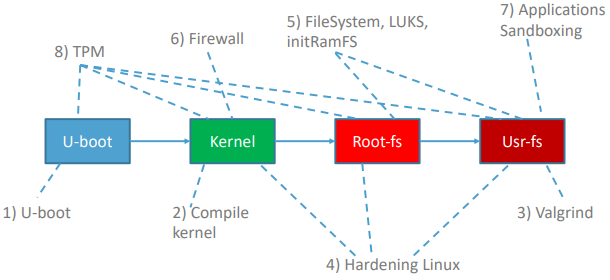
\includegraphics[width=\columnwidth]{img_0.png}
\end{figure}

\subsection{Attaques}
\begin{enumerate}
\item Attaques de surface
\begin{enumerate}
\item Utilisateurs des ports de debug
\item Connecteurs
\item Alimentations
\end{enumerate}
\item Vecteurs d'attaque
\begin{enumerate}
\item Réseau (Ethernet, Wifi)
\item Application
\item Port série
\item USB, I2C, Flash, Bluetooth, GPS, etc...
\end{enumerate}
\end{enumerate}
\subsection{Compilation pour nanopi}
Cross-compilation (ARM) effectuée sur un système x86/x64. Buildroot est le toolchain utilisé. Les éléments suivants sont compilés :
\begin{enumerate}
\item Bootloader
\item Kernel
\item Rootfs
\end{enumerate}
Puis les images sont copiées sur la carte SD
\end{document}